%%%%%%%%%%%%%%%%%%%%%%%%%%%%%%%%%%%%%%%%%%%%%%%%%%%%%%%%%%%%%%%%%%%%%%%%%%%%%%%
%
% witseiepaper-2005.tex
%
%                       Ken Nixon (12 October 2005)
%
%                       Sample Paper for ELEN417/455 2005
%
%%%%%%%%%%%%%%%%%%%%%%%%%%%%%%%%%%%%%%%%%%%%%%%%%%%%%%%%%%%%%%%%%%%%%%%%%%%%%%%%

\documentclass[11pt]{witseiepaper}

%
% All KJN's macros and goodies (some shameless borrowing from SPL)
\usepackage{KJN}
\usepackage[T1]{fontenc}
\usepackage{amsmath}
\usepackage{pgfgantt}
\usepackage{subcaption}
\usepackage{caption}
\usepackage{siunitx}
\usepackage{graphicx}
\graphicspath{{Images/}}
%
% PDF Info
%
\ifpdf
\pdfinfo{
/Title (Design Project)
/Author (Tristan Kuisis)
/CreationDate (D:201808300911)
/ModDate (D:200510121530)
/Subject (ELEN417/455 Paper Format, 2005)
/Keywords (Nothing)
}
\fi

%%%%%%%%%%%%%%%%%%%%%%%%%%%%%%%%%%%%%%%%%%%%%%%%%%%%%%%%%%%%%%%%%%%%%%%%%%%%%%%
\begin{document}

\title{Design Project}
\author{Tristan Kuisis
\thanks{School of Electrical \& Information Engineering, University of the
Witwatersrand, Private Bag 3, 2050, Johannesburg, South Africa}
}


%%%%%%%%%%%%%%%%%%%%%%%%%%%%%%%%%%%%%%%%%%%%%%%%%%%%%%%%%%%%%%%%%%%%%%%%%%%%%%%
%
\abstract{%The purpose of this document is to provide overview of the project undertaken from 16th of July to the 24th of August. 
Abstract Here}

\keywords{Keywords}


\maketitle
\thispagestyle{empty}\pagestyle{empty}


%%%%%%%%%%%%%%%%%%%%%%%%%%%%%%%%%%%%%%%%%%%%%%%%%%%%%%%%%%%%%%%%%%%%%%%%%%%%%%%
%




\section{INTRODUCTION} \label{sec:INTRODUCTION}

Over the last six decades, man has continuously propelled man made objects into space \cite{sputnik}. These objects have been said to exceed speed of $66 km/s$ \cite{fastestObject}, however, these extremely fast objects often leave the earths orbit and travel into outer space. Since the dawn of space exploration, many countries around the world have attemped, and in many cases, successfully deployed man made objects into the Earths upper atmosphere and into orbits around the Earth.

The organisations running these missions, in the early years, did not have sets of guidelines on how the missions should be carried out. In addition to this, there were many decades, during the Cold War era, that countries and organisations took extreme measures to make these missions a success. Many of the missions involved leaving many parts of the space craft in the Earths orbit \cite{spaceDebrisGuide}. Consequently, the number of debris orbiting the Earth grew over the years.
This was not thought to be an issue to the world at large as the belief was that space is immense and so there were no issues with using it as a dumping ground. It was not until the realisation by Kessler that the world began to worry \cite{Kessler}. This theory predicted that as the number of man made satellites (and other objects) in Earths orbit increases, so does the probability of collisions between them increase. When orbiting debris collide, the two objects can fragment (due to the excessive relative speeds with which the two objects travel at) and case multiple cascading collisions. This means that the debris orbiting the Earth would increase and result in greater difficulty for active space craft to undertake their missions.
Protecting active missions from this space debris is highly difficult as it is difficult to predict the density of objects in the specific orbit that the missions device should be in.

Guidelines were developed by NASA in the late 70's, however, this simply slowed the rate of introduction of debris and this did nothing to reduce the currently orbiting debris \cite{spaceDebrisGuide}. Recently, the United Nations General Assembly managed to get agreement between a number of countries to reduce the introduction of this debris \cite{debrisGuidelinesAgreement}.

There have been a number of methods in which to deal with this issue. The first is to protect the current missions from this debris, the first of these is to make use of a Whipple shield, this is simply an outer coating of space craft that is able to protect the craft against high velocity impacts of objects in outer space \cite{Whipple}. This shield is built to protect the craft from impacts from micrometeoroids in space.
This method falls short when the debris becomes large enough to penetrate the craft (and the Whipple shield), resulting in the destruction/damage of the craft.

A recent system is capable of removing debris from the Earths orbit, however, this is still in its early stages and has yet to prove highly effective \cite{removalSpaceDebris}.
The next method that systems currently make use of is object avoidance. This, however, is coupled with the fact that the location and trajectory of debris in orbit should be known and tracked. This forms the major task of this report.
Current solutions make use of either optical sensors which makes use of advanced telescopes in order to visually detect the debris. This system has a major drawback based on the fact that it can only be used during dawn and dusk hours \cite{OrbitalDebrisTechnicalAssessment,telescope,ZenithRanging}.
The second implementation makes use of radar techniques. This is the method which is implemented in this system.

This report begins with explaining the background to the task given, this includes an explanation of how the radar system works (in principle).
This is then followed up with a description of the space debris as well as a number of calculations on the characteristics of this debris.

Once the debris has been characterised, current implementations used for this application are analysed and compared.  

*** Need more here on the structure of the report.
% in the document: a-technical-assessment there is an image which breaks down all of the types of space debris

\subsection{Background} \label{sec:Background}
Due to the increase in Earth-to-Space launches currently taking place globally, it has become pertinent for space agencies to determine the optimal launch times and characteristics of their missions in order to avoid space debris currently in orbit. This signals the requirement of systems that are capable of detecting this debris from the ground.
The aim of the system is such that it is able to detect and track this space debris with the use of phased array radars.
A number of assumptions are created in order to carry out the design of this system, these are discussed in the following sections.
The idea behind radars is such that an electromagnetic (EM) pulse is created and then launched in a specified direction, this EM wave travels in the specified direction and comes into contact with an object. This object then proceeds to scatter these EM waves in a number of directions. The characteristics of this scattering are discussed in minimal detail in order to characterise the object. 
The system is then used to receive these scattered EM waves and an assumption is created in order to detect and then analyse the signals to identify the object and determine its parameters.
It is the design of this system that is undertaken throughout this report. 


\subsection{Space Debris} \label{sec:SpaceDebris}
As discussed in section~\ref{sec:INTRODUCTION}, space debris in Earths orbit has been increasing for many decades, this is mainly due to space missions with poor regulations on the material that is allowed to stay in Earths orbit.
The majority of space debris currently is made up of man made air craft components, this includes objects such as: funcioning space craft, non-functional spacecraft, rocket bodies, exhaust products, objects created through deployment operations, and products of deteriorated space craft \cite{OrbitalDebrisTechnicalAssessment}.
Consequently, a large amount of this debris is made up of metallic materials as these materials make up the majority of the space crafts' components.
It has, in the past \cite{Spacex}, been difficult and costly to retrive the components which were used to get the space craft into orbit, this is a major contributer to the material.
This debris can occupy a number of regions within the Earths orbits and this changes its characteristics.
The current scope of the project is that it should be capable of tracking space debris that is within the Low Earth Orbit (LEO). This orbit is defined to be approximately $160 km$ to $2000 km$ altitude above the Earths mean sea level.


\subsubsection{Space Debris Trajectory Characteristics} \label{sec:SpaceDebrisTrajectoryCharacteristics}

The second definition of these orbits is baed on orbital mechanics, this states that if an object is within an orbit, then it will have a corresponding velocity.
This is illustrated by equation~\ref{eqn:OrbitalVelocity}. 

\begin{equation} \label{eqn:OrbitalVelocity}
    V_{Object} = \sqrt{\frac{G M_{Earth}}{r_{Earth} + r_{Altitude}}}
\end{equation}
Where:
\begin{itemize}
    \item $V_{Object}$ is the radial velocity of the object
    \item $G$ is the gravitational constant ($6.67408 \cdot 10^{-11} m^3 kg^{-1} s^{-2}$)
    \item $M_{earth}$ is the mass of the Earth ($5972 \cdot 10^{24} kg$)
    \item $r_{Earth}$ is the mean radius of the Earth
    \item $r_{Altitude}$ is the altitude of the object above the mean radius of the Earth
\end{itemize}

This allows for the simple calculation of the minimum and maximum orbital speeds expected from the objects which correspond to the maximum altitude and minimum altitude respectively. These are illustrated in table~\ref{tab:ObjectParameters}. The velocity in the table is stated as a tangential velocity as it is assumed that the radial velocity of the object is zero. If an object has a radial velocity componenet, then this implies that it is changing orbits (an object in a specified orbit will have zero radial velocity) and this is either taking place due to a force acting on the object (man made) or it is experiencing a force due to the Earths atmosphere. The vectors which explain this movement of an object is illustrated in figure~\ref{fig:ObjectVelocityVectors}.

\begin{center}
    \begin{figure}
        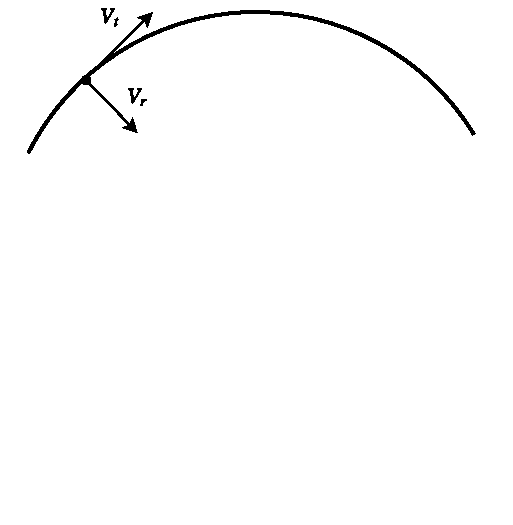
\includegraphics[width=\textwidth]{Vectors.pdf}
        \caption{Object Velocity Vectors}
        \label{fig:ObjectVelocityVectors}    
    \end{figure}
\end{center}

The objects orbiting within these ranges have corresponding periods (amount of time it takes for an object to orbit around the Earth once), this means that an object in the lower orbit has a higher period than that of the higher orbits. The periods for the two limits of the LEO objects are also found in table~\ref{tab:ObjectParameters}.

Based on a number of physical limitations, the system implemented will only be capable of detecting the space debris once it appears within the field of view (FOV). The FOV is discussed in section~\ref{sec:FieldOfView}. Figure~\ref{fig:ObservableCharacteristics} illustrates the system and how its relation to the Earth. 
The inner circle represents the Earths surface and point P represents the position of the system on the Earths surface.  
The outer circule represents the path of an object orbiting the Earth.
The lenghts in this image are not to scale and do not represent the real situation, however, this is used for illustrative purposes.
It is highly important to determine the amount of time it takes from when the object first enters the systems FOV, until the point where it exits the systems point of view.
In this case it is assumed that the object travels directly over the boresite of the system and so it will take the maximum amount of time to travel over the field of fiew. In most cases, the objects do not travel directly over the FOV, and will therefore not be within the FOV for a reduced amount of time.
This illustrates the system in order to create a few starting assumptions/criteria for the system.
As can be seen in this image, the angle that is measured can be taken from two different reference points: the center of the Earth and the point P. Based on this, it can be seen that the angles that these two points create are different. This implies that if one were to calculate the maximum distance that an object can be detected (assuming a maximum FOV angle from point P), one cannot make use of the angle $\alpha$ and the distances of this arc as it would not represent the actual distances of the objects because the circle that the objects orbits around is different to the circle that is assumed the system makes use of.
Numbers $1$ and $3$ represent the points at which the object enters and leaves the FOV, and point $2$ represents the position of the systems zenith.

\begin{center}
    \begin{figure}
        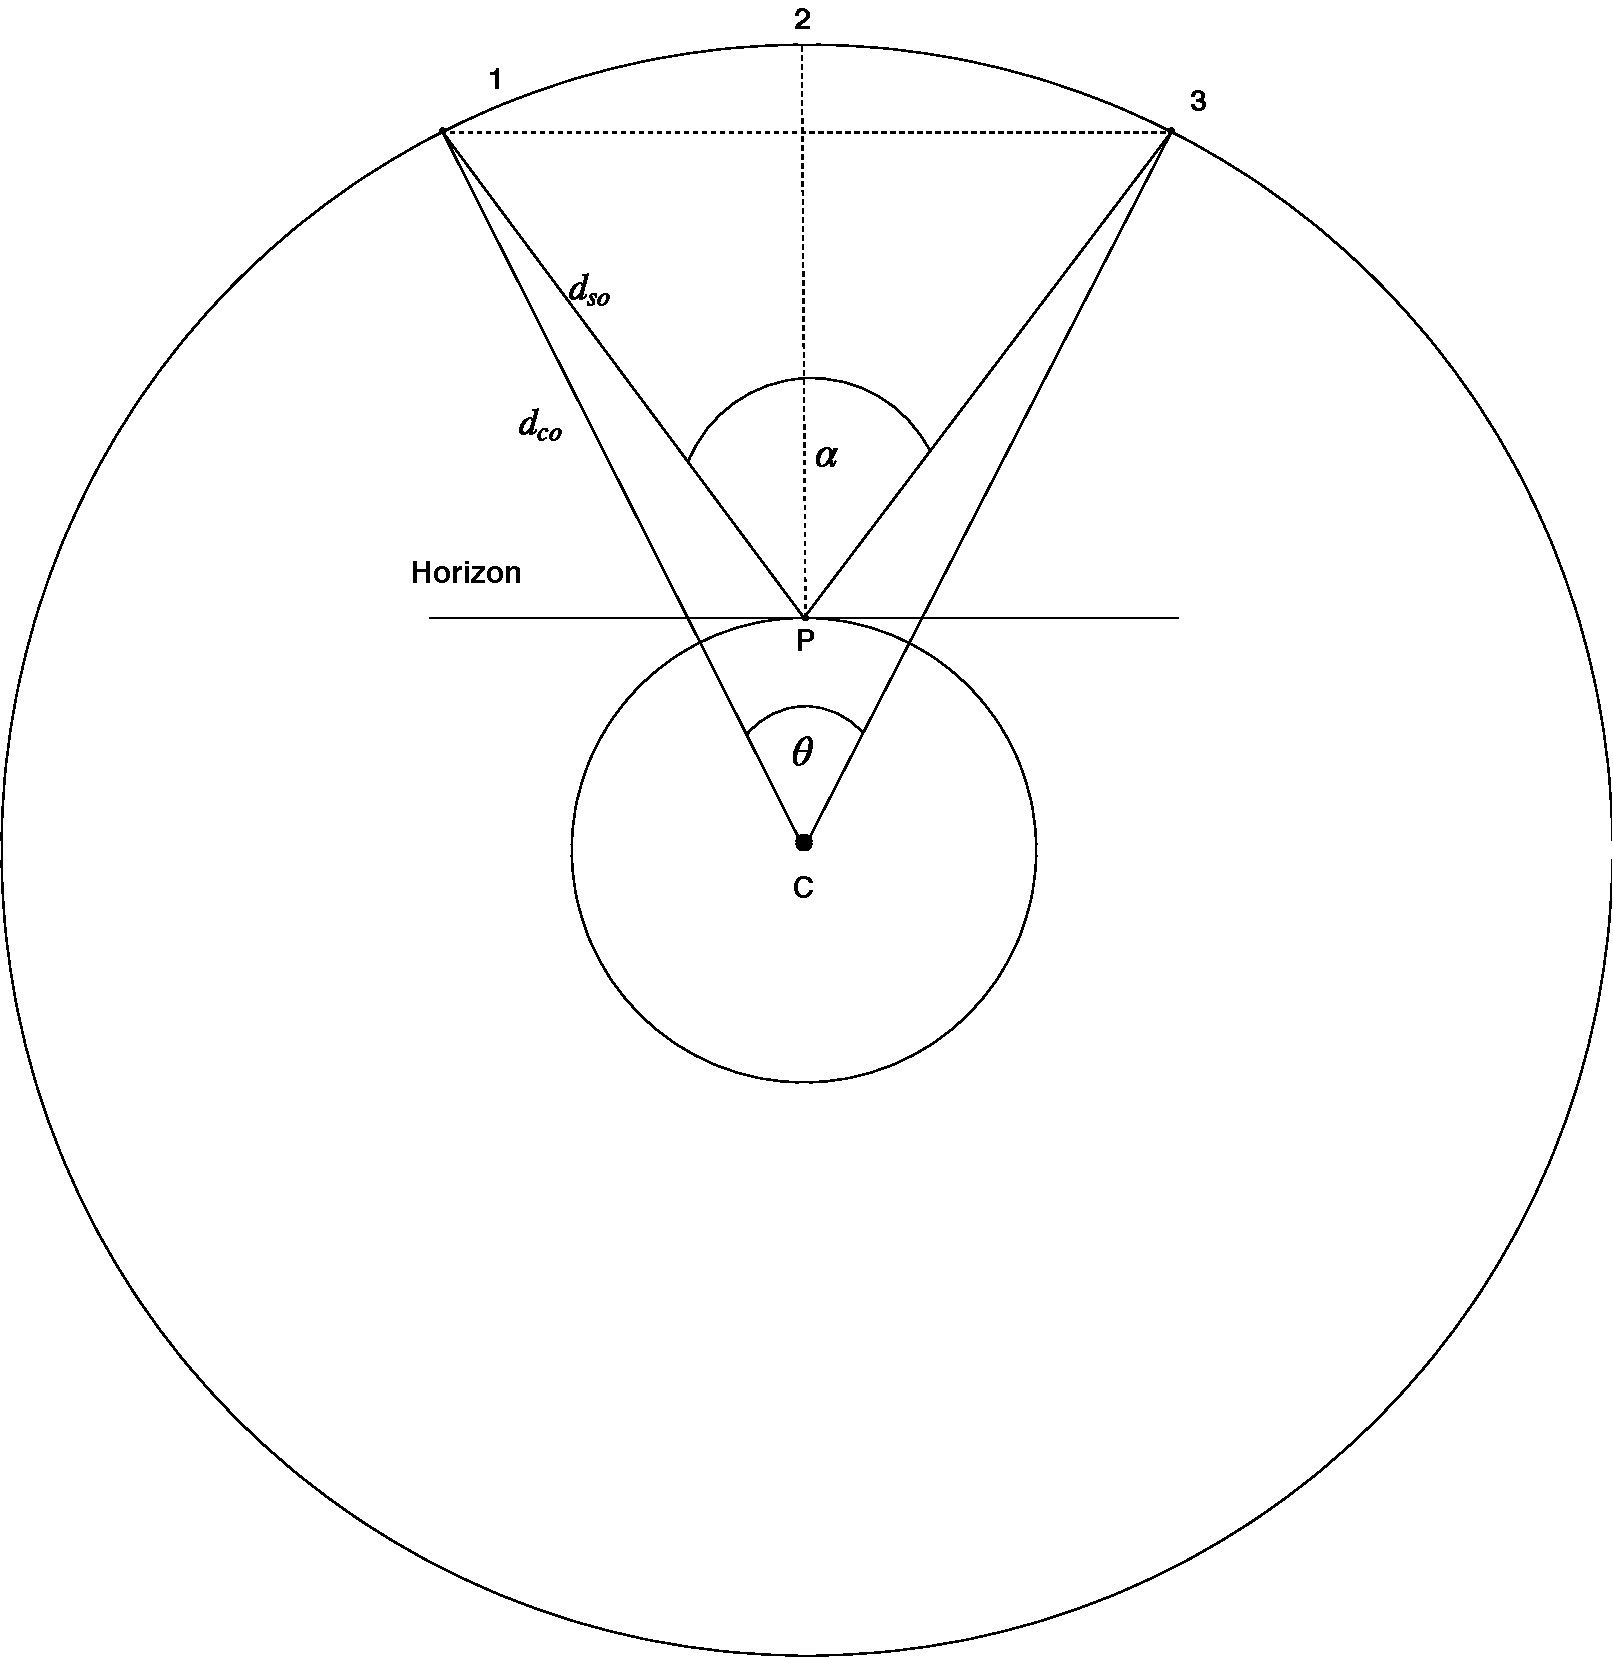
\includegraphics[width=\textwidth]{ObservableCharacteristics.pdf}
        \caption{Observable Characteristics}
        \label{fig:ObservableCharacteristics}    
    \end{figure}
\end{center}
The calculations in this section make use of a specified mean Earth radius, this implies that the observer is positioned at approximately sea level, this is unlikely to be the case for the placement of the system, however, the maximum altitude of feasible locations within South Africa are unlikely to exceed $\sim 1500 m$, this change in distance will provide a negligible difference to the calculated values.


Based on the movement of objects in differing orbits, it can be seen that objects in higher orbits move slower than those in lower orbits.
The objects move with a specific velocity, as illustrated in table~\ref{tab:ObjectParameters}, this is measured in linear velocity, however, it is also important to represent the motion of these objects with the use of their angular velocity, the angular velocity is simply found with the use of equation~\ref{eqn:AngularVelocity}.

\begin{equation} \label{eqn:AngularVelocity}
\omega = \frac{v}{r}
\end{equation}
Where:
\begin{itemize}
    \item $\omega$ represents the angular velocity of the object (Radians per second)
    \item $v$ represents the linear velocity of the object
    \item $r$ represents the distance from the observer to the object
\end{itemize}


Once this has been estimated, it is important to evaluate the angle travelled by the object as seen from the observation point ($\alpha_{p}$). This is measured over a period of time ($\Delta T$) and the angular velocity calculated above ($\omega_{P}$) is used, this is found in equation~\ref{eqn:AngularVelocityP}

\begin{equation} \label{eqn:AngularVelocityP}
    \omega_{P} = \frac{\theta_{P}}{\Delta T}
\end{equation}
Where:
\begin{itemize}
    \item $\omega_{P}$ is the same as before
    \item $\theta_{P}$ represents the angle of the object seen from the observation point
    \item $\Delta T$ represents the amount of time that it takes the object to traverse the angle
\end{itemize}

This now allows for the calculation of the linear velocity of the object as seen from the observation point (it is the same if the center of the Earth is used as the reference point). This velocity is calculated with the use of equation~\ref{eqn:LinearVelocity}.

\begin{equation} \label{eqn:LinearVelocity}
    v = \omega_{P} h
\end{equation}
Where:
\begin{itemize}
    \item $v$ is the linear velocity of the object (m/s)
    \item $\omega_{P}$ represents the apparent angular velocity of the satellite (Radians)
    \item $h$ represents the altitude of the object
\end{itemize}


The use of the two equations above require the values for the amount of time that it takes for an object to enter the FOV of the system and exit it again. This is found with the use of equation~\ref{eqn:ObservableTime} \cite{ObservableTime}.

\begin{equation} \label{eqn:ObservableTime}
    t_{t} = \frac{r^{\frac{3}{2}}}{\sqrt{GM}} (\pi - 2E - 2 asin(\frac{R}{r} cos(E)))
\end{equation}
Where:
\begin{itemize}
    \item $t_{t}$ is the amount of time that an object is in the FOV of the system
    \item $r$ is the geocentric distance of the object (distance of the object above mean sea level)
    \item $G$ is the gravitational constant
    \item $M$ is the mass of the earth
    \item $E$ represents the elevation of the object above the horizon of the system
\end{itemize}

The elevation of the system is important as it relates to the FOV of the system. The two are interrelated by the fact that the elevation angle is the complementary angle of the maximum FOV of the system. This implies that if the elevation of the system is known, then the FOV of the system can be calculated.

In table~\ref{tab:ObjectParameters}, the elevation angle is assumed to be approximately $60^{\circ}$, this is a first estimate of the FOV of the system, further analysis of the system FOV of the system can be found in \ref{sec:FieldOfView}. This elevation angle creates a maximum amount of time that the object is visible. This implies that the object travels directly over the boresight of the system. In most circumstances, the objects will not travel directly over the boresight and will therefore be within the FOV for less time than stated in this table.

This creates the ability to calculate the observed velocity of the object as it passes over the FOV of the system, this is illustrated in figure~\ref{eqn:ObjectVelocity}.

\begin{equation} \label{eqn:ObjectVelocity}
    v = \omega_{P} h
\end{equation}
Where:
\begin{itemize}
    \item $v$ is the linear velocity of the object (m/s)
    \item $\omega_{P}$ represents the apparent angular velocity of the satellite (Radians)
    \item $h$ represents the altitude of the object
\end{itemize}


In addition to this, with an assumed elevation angle, the expected distances for the objects can be found, these are calculated making use of equation~\ref{eqn:ObjectDistances} \cite{ObservableTime}.


\begin{equation} \label{eqn:ObjectDistances}
    \rho = R (\sqrt{\frac{r^2}{R^2} - (cos(E))^2} - sin(E))
    \end{equation}
Where:
\begin{itemize}
    \item $\rho$ is the slant distance from the system to the object
\end{itemize}
This equation is important as it provides another criteria for the system, that of the maximum range that is required to be detected by the system. These become important for the Radar Range Equations (RRE) in section \ref{sec:SNRRRE}.


\begin{table}
    \begin{center}
        \begin{tabular}{ c c }
            \hline 
            Minimum Object Altitude & $160 km$ \\
            Maximum Object Altitude & $2000 km$ \\
            Minimum Object Slant Distance & $184 km$ \\
            Maximum Object Slant Distance & $2223.8 km$ \\            
            Minimum Object Tangential Velocity & $6897.4 m/s$ \\
            Maximum Object Tangential Velocity & $7807.9 m/s$ \\
            Minimum Angular Velocity & $0.0034 rad/sec$ \\
            Maximum Angular Velocity & $0.0488 rad/sec$ \\
            Elevation Angle (assumed for illustration) & $60^{\circ}$ \\
            Angle (Measured from Zenith) & $30^{\circ}$ \\
            Maximum Observable Time & $323.37 s$ \\
            Apparent Angular Velocity & $0.0032 rad/sec$ \\
            Minimum Linear Velocity & $518.14 m/s$ \\
            Maximum Linear Velocity & $6476.8 m/s$ \\
        \end{tabular}
        \caption{Object Parameters}
        \label{tab:ObjectParameters}
    \end{center}
\end{table}

\subsubsection{Space Debris Physical Characteristics} \label{sec:SpaceDebrisPhysicalCharacteristics}
Now that a number of key characteristics of the movement of the objects have been calculated, it is important to detail the sizing and physical characteristics of the objects that are evaluated.

There are multiple ways in which to model the space debris that is being tracked. This includes parameters such as: electron density, ion composition, electron drift velocity, etc. This in depth analysis of the debris is out of the scope of the project and a few simplifying assumptions are chosen for this section of the report.
The first of these is to assume that the system is only required to detect \textit{hard} targets, this refers to the fact that the object is a solid and has a predictable characteristic when reflecting the EM waves incident on it. The \textit{soft} targets include ionospheric plasma present in the atmosphere, these targets are not important to this report \cite{softTarget}.  

Based on current implementations of space debris trackers, an assumption is created here that the minimum RCS of an object is assumed to be that of $10 cm$ in diameter.
As discussed in the above section, the objects in question are assumed to lie within the LEO, objects that are below this range experience force due to the atmosphere and therefore will slowly lose orbital velocity and will eventually fall into the Earths atmosphere and (commonly) burn up in the process.
The majority of the objects lie within the $500 km$ to $1000 km$ altitude band, after this point, the density of objects decreases \cite{ObjectInformation}. 

The information provided in the sections above create a baseline with which to design the system.



% What is an Antenna?
% What is an array?
% What is an antenna array?
% What is space?
% What is space debris? (How did it get there? why is it there? what is it made up of? where is it in space? how is it moving in space? is it bad/good? can we remove it? should we remove it, why? why do we care? who wants to know? fastest moving debris? how often do they come into contact with each other ? what happens when they come into contact with each other? can we protect against it? how is it currently being tracked?)
% What are orbits?
% What is lower earth orbit? Geostationary orbit?
%  What is the atmosphere? (Range? made up of?)
%  What is the ionosphere? (Range? made up of? characteristics? EM characteristics? How fast can things move through them? )
%  current technology? radar and telescopes? advantages and disadvantages of these technologies?

% The nature of an Incoherent Scatter Radar system is such that it directs electromagnetic energy into the earths "surrounding area"(ionosphere?); it highlights irregular characteristics present in this space. The energy that is transmitted is then reflected off of these irregularities and returns back in the direction of the system.
% The system has the ability to create a narrow beam which transmits energy, this energy is then sterred (electronically) within the bounds of the system. Steering can be done in azimuth, elevation, and intensity. 


\subsection{Current Implementations}
The baseline for this project is built upon the system created by Leo Labs \cite{LEOLABS}. The Leo Labs system makes use of two systems that are currently installed. The first of these is the Advanced Modular Incoherent Scatter Radar (AMISR), this is locaed in Resolute Bay, Canade, it makes use of an array of crossed-dipole antennas that are electrically phased. This implies that the system is electronically steerable. It operates in the frequency range of $430 MHz$ to $450 MHz$ and has a pulse width of approximately $2 \nu s$ \cite{AMISR}. A number of important parameters can be found in \cite{AMISR}, this is a system which closely resembles the major requirements for this system.
The second system in use by LEOLABS is the Midland Space Radar (MSR), this system is located in Texas and is commissioned by LeoLabs, this system is capable of detecting objects as small as $10 cm$ in diameter. It is not specified whether this value is a Radar Cross Section  (RCS) or the physical size of the object.
A number of other implementations have been used (not through Leo Labs) which make use of other technologies and are capable of detecting smaller objects \cite{EISCAT, SIMO, telescope, BeamForming, OrbitDetermination, PlanarArray}. A number of these papers are made use of to design the system in this report.


\section{TECHNOLOGY} \label{sec:TECHNOLOGY}
Based on the research on previous implementations of this technology, it appears as if the best solution to this problem is to make use of multiple antennas such that they form an array that can be electronically sterred in a specified direction.
The basic functionality of the system is that of a radar where the array sends out a pulse through the use of an EM wave which then bounces off of the object and this echo is detected with the use of an array, once this reflection has been received, sampled, and processed, the system is capable of determine a number of characteristics of the object.

The following sections detail the different implementations of this sytem and determine the advantages and disadvantages of each choice.
The system, as an overview is made up of the following components illustrated in figure~\ref{fig:SystemOverview} \cite{radarHandbook}.

\begin{center}
    \begin{figure}
        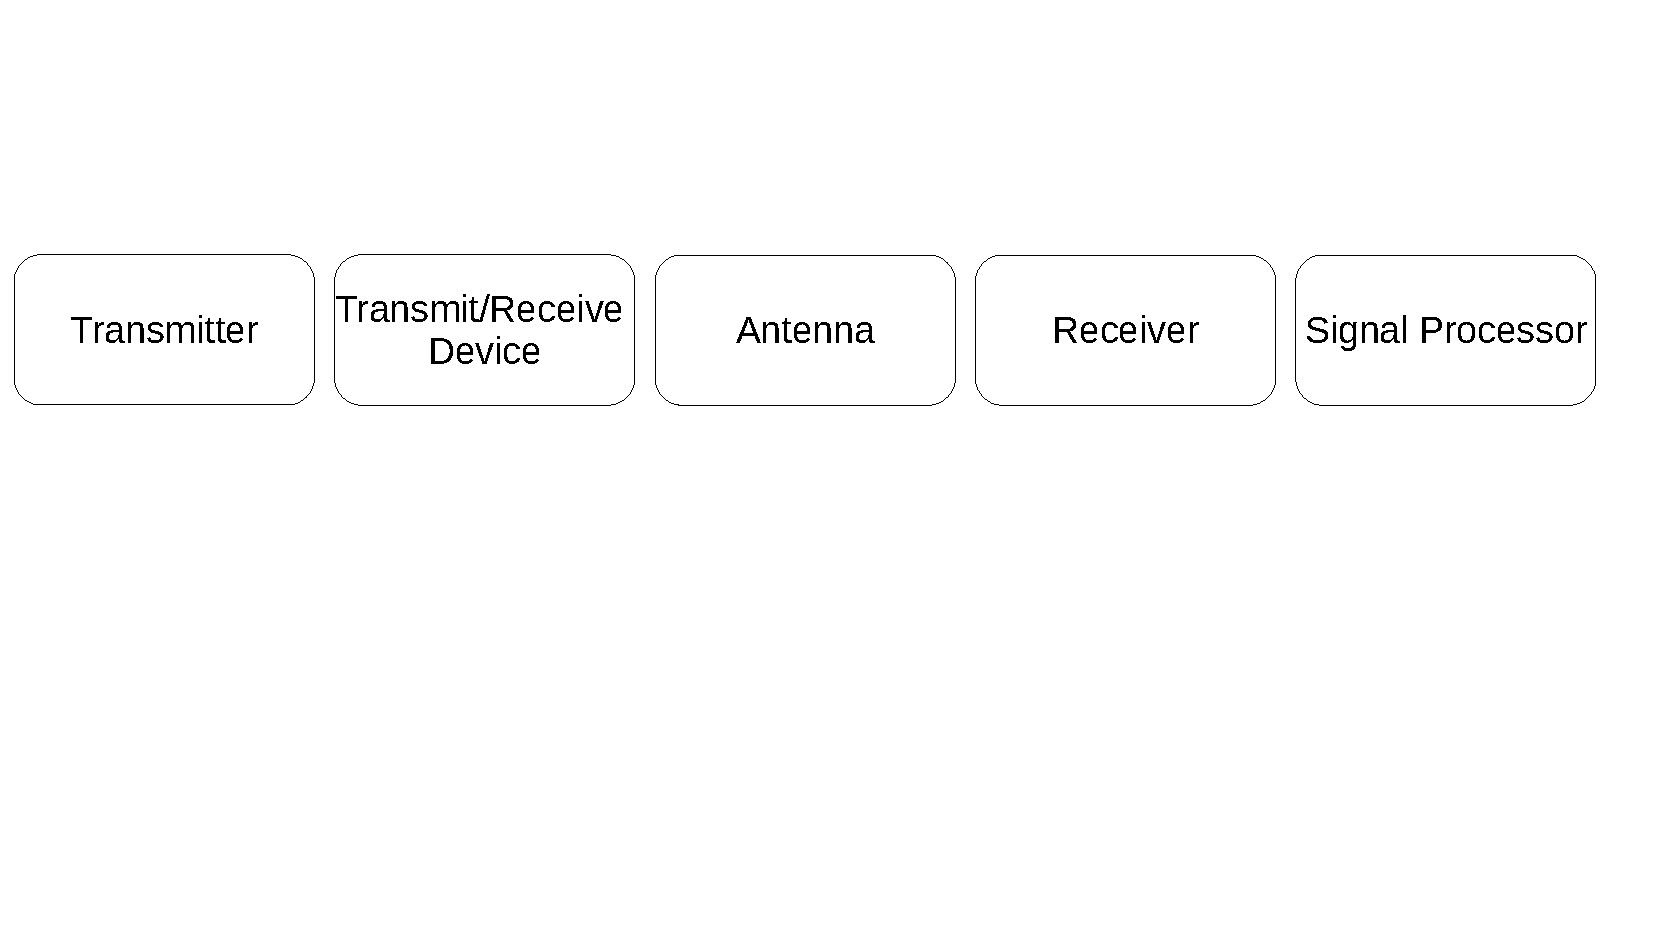
\includegraphics[width=\textwidth]{SystemOverview.pdf}
        \caption{System Overview}
        \label{fig:SystemOverview}    
    \end{figure}
\end{center}
These components perform the major tasks of the system, they are each discussed in detail in their own sections, however, before that can take place, these components are used to perform a specific action in order to detect the space debris, sections~\ref{sec:OptimalFrequency}, \ref{sec:ArrayStructure}, \ref{sec:ContinuousWaveandPulsedWave}, \ref{sec:RadarFunctions}, and \ref{sec:SNRRRE} introduce the theory behind the operation of this system. The choices for these sections are directly linked to the type of devices and components seen in figure~\ref{fig:SystemOverview}.
The first highly important parameter of the system is the frequency at which it will operate as this is dependent on a number of factors. This is discussed in section~\ref{sec:OptimalFrequency}.



% \subsection{System}
% The system can be illustrated with the use of the design slides. This illustrates the entirety of the system.
% The elements which make up the system include:

%     * Transmitter
%     * T/R Device
%     * Antenna
%     * Receiver
%     * Signal Processor

% Each of these items will have their own section.
% However, there will be sections which discuss other components/characteristics of the system.

% Section on EM waves and how they are created, influenced, propagated, polarized, phase shifted, their spectrums, superpositioned, 
% Introduce the simple kinds of polarization and then reference later parts in the report that the waves will be affected by the structure of the antenna and the array as well as the atmosphere.

\section{Optimal Frequency} \label{sec:OptimalFrequency}
A number of constraints exist for the frequency of operation of the system, these range from economical, political, technical, and physical. These constraints and the reasons behind the final choice of frequency is discussed within this section.

\subsection{Technical and Physical Limitations} \label{sec:TechnicalandPhysicalLimitations}

The first limitation of the system is the fact that the ionosphere attenuates frequencies from specific frequency range. This is important as it is known that there are two frequency windows at which EM waves penetrate the ionosphere without excessive attenuation \cite{ObjectInformation}.
These frequency windows have a high transmission coefficient for frequencies within the $1 cm$ through to the $1 m$ wavelength range, this implies that these frequency bands are highly useful for transmitting EM waves through the Earths atmosphere as the attenuation is low \cite{frequencyAttenuation}. Frequencies outside of this window (with a few exceptions to some of the visible light spectrum), are closed due to ionospheric attenuations and reflections (at larger wavelengths) and also attenuate due to resonances created by molecules in the atmosphere (at lower wavelengths) \cite{frequencyAttenuation}.  
If the wavelength of the EM wave is within the bands above, then the attenuation can be considered neglible \cite{ionosphereAttenuationStandard}, \cite[p~.15,124]{radarHandbook}. It is apparent that frequencies within this range provide an attenuation of less than $10^{-2} db/km$ which is negligible.
Based on these assumptions, the frequency band of interest lies within the $200 MHz$ up to $1 GHz$, after $1 GHz$, the atmospheric losses increase accordingly.

The elevation angle of the system is also a contributing factor to the loss of the system as this determines the \textit{volume} of atmosphere that the EM waves travel through to rech the target. An increasing elevation angle results in a lower two-way loss, this implies that in the case that the system directs its beam directly upwards (towards the zenith), this is the direction with the least loss per unit distance \cite[p~.70]{elevationLoss}. This is highly beneficial for the system as it is normally directed upwards and has a FOV that does not greatly increase the \textit{volume} of atmosphere the EM wave has to encounter.

Included in this technical choice is that of currently implemented systems. Many of these operate within the $400 MHz$ to $500 MHz$ frequency bands.
The amount of electrical power required for these systems can often be in the megawatt range and components capable of supplying this power in the $GHz$ range become prohibitively expensive, this further backs up the choice for a lower frequency.

The frequency that is transmitted from the radar is likely to be different to the frequency that is returned by the object, this is in part due to the Doppler shift phenomenon. The maximum frequency shift created by the Doppler shift is evaluated with the use of equation~\ref{eqn:Doppler}. This implies that the maximum expected Doppler frequency shift is unlikely to exceed $\sim 50 kHz$. This value is created with the assumption that the frequency is chosen to be $1 GHz$ (which creates the maximum frequency shift) which is the upper bound of frequencies that can be selected from.


\begin{equation} \label{eqn:Doppler}
    f_{d} = \pm \frac{2 v_{r}}{\lambda}    
\end{equation}
Where:
\begin{itemize}
    \item $f_{d}$ is the frequency shift due to the maximum linear velocity of an object
    \item $v_{r}$ is the maximum linear velocity of an object
    \item $\lambda$ represents the wavelength of the frequency of choice.
\end{itemize}

This assumed Doppler shift implies that the frequency bandwidth should accomodate at least $100 kHz$ on either side of the centre frequency.
The Doppler frequency shift of the designed system is discussed in more detail in section~\ref{sec:RadarFunctions} where further analysis on the required bandwidth is also required: the bandwidth of the system is dependent on a number of components.


The frequency choice is highly dependend on the locality of the system and the current frequency usage by other parties. ***


\subsection{Political and Economical Limitations} \label{PoliticalandEconomicalLimitations}

In addition to the reasons stated above, a further factor that affects the frequency band choice are those frequencies available by the systems regulator. The current communications authority of South Africa is run by ICASA \cite{ICASA}.
ICASA keep an updated list of the currently used frequency bands and the regulations that the operators should adhere to \cite{frequencyAllocation}, this document is used in order to determine the optimal frequency band.

The frequency allocation within a country is highly regulated, and as such it becomes costly to demarcate specified frequency bands for specific uses.
The first criteria for the choice of a frequency band is the current usage of the frequency band, the request for in-use bands can expand the budget of the system greatly.

The method used to determine the optimal frequency band is to first define the search range, this is given in the above section ($200 MHz$ to $1 GHz$), from this point, the frequency bands that are commonly allocated to astronomy research are narrowed down. The frequencies which lie within this area of interest are: $406.1 - 410 MHz$ and $606 - 614 MHz$. 




It appears as if the last frequency allocation happened in 2013.
The next one is up for approval and is in draft stage. There are a number of bands which appear to be moving and this can affect things.

[This](https://www.icasa.org.za/legislation-and-regulations/national-radio-frequency-plan-2013) appears to contain the 2013 allocation.

Frequency allocation by [SKA](https://www.ska.ac.za/about/astronomy-geographic-advantage-act/)

The chosen frequency at this point is: 610 MHz.
The frequency on either side of the band is 4 MHz.
Wavelength: 0.4918 m
3/4 wavelength: 0.3689 m
1/2 wavelength: 0.2459 m
1/4 wavelength: 0.12295 m

\subsubsection{Astronomy Geographic Advantage Act}

The minister has the ability to declare any area or part of an area in the Province of the Northern Cape as an astronomy advantage area. This implies that an area, which is technically advantagous to the functioning of the system can be demarkated by this act.
A number of proccesses are required to take place for these areas to be allocated to the system. These include a number of considerations for: local businesses, affected agricultural participants, environmental impacts, nearby electrical and radio interference.

The act allows for specific frequencies to be used (regardless of the current frequency allocation by ICASA) as long as it is assessed by the procedures required by the SKA. Permits can be issued by the act and they are then allowed to operate within the permitted areas. These permits include exemptions for the frequency spectrum that is allowed to be used and the permitted transmission characteristics.

The current situation with ICASA is such that there is a 50 mW maximum allowable broadcast power. However, with the use of the AGA, the TV transmission services are limited in the Northern Cape.

The band chosen is currently allocated ot the radion astronomy service on a primary basis.








The radar equation forms the initial stage for the design process.

Primary functions:

    * Impedance transformation (free-space fields to guided waves)
    * Propagation-mode adapter (free-space to guided waves)
    * Spatial filter (radiation pattern - direction-dependent sensitivity)
    * Polariation filter (polarization-dependent sensitivity)

The antenna is used to fix the mismatch between free-space and the rest of the system.
Intrinsic impedance of free-space: $n_0 = E/H$
$n_0 = sqrt(u_0 / e_0) = 120 * pi ~= 376.7 \Omega$

Characteristic impedance of tx line, $Z_0 = V/I$ (typically $50 \Omega$)



Make use of [this](https://etd.ohiolink.edu/!etd.send\_file?accession=ohiou1345227397\&disposition=inline) to speak about the axial ratio and how polarization is done.

\subsection{Array Structure} \label{sec:ArrayStructure}

\subsubsection{Monostatic versus Bistatic} \label{sec:MonostaticvsBistatic}

There are two major radar configurations that are used. 

\subsubsection{Bistatic} \label{sec:Bistatic}

The bistatic configuration makes use of a separate transmitter and receiver for the system. The two components are placed at differing locations and the separation between the components is required to be sufficiently large in terms of the angles or ranges that they present.
This implies that the two systems, in the case of Earth-to-Space transmission, are required to be geographically (in the order of kilometers) far apart \cite{bistaticNato}.
The transmitters in these systems generally transmit power in the range of kilowatts to megawatts, this is in order to increase the signal-to-noise (SNR) of the system as there is a significant amount of energy lost in the energy transfer process. The receiver on the other hand, works with milliwatts to nanowatts as it receives this greatly reduced power that is reflected from the objects in question. The bistatic system provides a concenient method of separating out the two systems such that it becomes increasingly difficult to damage the receivers equipment from the high power generated by the transmitter.

\subsubsection{Monostatic} \label{sec:Monostatic}

The other, more commonly used system, is the monostatic configuration. This bundles the transmitter and receiver together on the same antenna/antenna array. In this case, a system is required such that the transmitted and received signals are isolated from eachother when they interact with the system. The isolation can be carried out in different ways, a circulator or a switch commonly achieves this. These components are discussed in a later section ***. In the monostatic configuration, the transmitter and receiver do not operate at the same time which greatly simplifies the switching apparatus.

\subsubsection{Comparison} \label{sec:Comparison}

The configuration implemented is the monostatic as it provides a lower cost alternative to the bistatic configuration. It has the added benefit of only requiring one piece of land for the system. The system cost is also reduced by the fact that only one set of antennas are required.
The bistatic configuration is easier to implement with regards to the protection systems for the receiver, however, this benefit does not out weigh the monostatic systems advantages. The bistatic systems also require a significant amount of communication between the two systems and this can increase the cost of implementation, most notably when the distance between the two systems is large and communication mediums can become prohibitively expensive.

\subsection{Continuous Wave and Pulsed Wave} \label{sec:ContinuousWaveandPulsedWave}

The two commonly used transmission systems are the continuous wave and the pulsed wave, these two systems are also linked to the choice on the system configuration.
This implies that if the monostatic configuration is used, then the continuous wave transmission system is not available.

\subsubsection{Continuous Wave Transmission} \label{sec:ContinuousWaveTransmission}

The continuous wave transmission system, as the name indicates, has the transmitter functioning $100\%$ of the time, which implies that the receiver also functions all of the time. The continuous wave transmission system, as indicated above can only be used by the bistatic configuration. 
A unique characteristic of the continuous wave system is that it is unable to determine the electromagnetic (EM) waves round-trip time as there is no set begin and end time of transmission. This can be solved with the use of modulation on the wave, this implies that the receiver is required to know all of the characteristics of the transmitters waveforms ahead of time if it is to determine round trip times \cite[p.~20]{radarHandbook}.

\subsubsection{Pulsed Waveform Transmission} \label{sec:PulsedWaveformTransmission}

The second mehtod of EM wave transmission makes use of pulses, these occur periodically and their duration is commonly over a short period of time. This system is commonly used in tandem with a monostatic configuration and this provides the isolation between the transmitter and receiver circuitry, the circuitry to isolate these signals is still used.
Following the EM wave pulse, the receiver is set to record the resulting EM waves that are returned in the form of echoes after it has reflected from the objects in question. The determination of the pulse length and the period between pulses (the interpulse period (IPP))is discussed further in the report ***. The pulse repitition is also highly pertinent to the observable time window of debris, this will be discussed in section ***.

Need image here which describes how the pulses are placed with respect to time.

The pulse repetition frequency is related to the maximum distance that the system is able to detect objects, this is related to the observable area of the system and the furthest distance that the system can detect an object. This is discussed in section *** and section ***.

The following image represents a case where a pulse is sent outwards and is then followed by, a period of time later, a corresponding echo pulse.
The period between the pulse and the echo can be used to determine the altitude that the object has.
In order to detect the pulse, the time between each sample should be no less than the pulse width of the transmitter (this should be elaborated on... get the info from: \cite[p.~21]{radarHandbook})

Think about echoes that come back after the next pulse is fired, this can be from targets that are past the 2000 km range. These need to be dealt with. One way is to define a SNR that will rule out these cases. Another case is to throw out any echoes that happen before one is expected to have returned (based on the minimum altitude required to be detected). 
This issue is known as a range ambituite (\cite[p~.22]{radarHandbook})

*** Include calculation of the pulse width and the corresponding bandwidth if requires. Stuffies for this can be found on page 65

\subsection{Threshold Detection} \label{sec:ThresholdDetection}

In order to detect a signal, the received signals' power is required to be above a specific threshold. This threshold is defined as the level at which all sources of noise are incorporated. When an object is detected, the signal level is required to rise above this threshold and this is then considered a successful detection.

There are cases, based on the fact that noise is inherently a random variable, that the noise level can exceed the threshold set by the system. This is observed as a false alarm.
This implies that there are cases where the targets echo in addition to the noise are capable of being below the threshold, this is when the noise in the system is low, so the addition of the echo is not large enough for the system to detect the object.
These two cases are highly unlikely, however, cannot be ignored as they are based on the probabilities of the entire system.

These probabilities are given as two variables: the probability of detection ($P_{D}$), and the probability of false alarm ($P_{FA}$). The probability of detection is the probability that an object-plus-noise exceeds the threshold applied to the system. The probability of false alarm is the probability that the noise (from all components of the system) will exceed the threshold.
The best case scenario for these two variables are: 
$P_{D} = 1$
and
$P_{FA} = 0$

These values are idealistic and so the correct threshold value is required to be set such that the system can operate as close to these values as possible.
When the threshold is increased the probability of false alarm will decrease, however, so will the probability of detection. When the threshold is decreased, the probabilities of both variables increase. A trade-off is required here to determine the optimum threshold level.

There is one way in which to increase the probability of detection while lowering the probability of false alarm, this is achieved by increasing the targets signal power (it should be noted that the signal power should be increased relative to the noise power). 
<!-- If the noise power increases in ratio with the overall power, then this will not work -->

The importance of Doppler should not be underestimated. Doppler shift is important as it can be used to reduce the effects of clutter in the viewing area, it is also able to perform measurements to detect if there is more than one object in the viewing area (in the same range). The removal of clutter from view of the system is achieved with Doppler by the fact that clutter is not moving and thus will have a no frequency shift.

\subsection{Resolution} \label{sec:Resolution}

The resolution of the system has three components: the ability to distinguish between objects that are different distances away from the system, have differing angles with respecto the the system, and have differing Doppler frequencies.

The first of these, the range resolution, determines if you are able to discren two objects that are in eachothers vacinity.
The range resolution is defined by:
$\delta R = \frac{c \tau}{2}$

This implies that if the pulse width of the signal is 1us, then the range resolution of the system is $150 m$. This implies that if the pulse width is decreased, then the range resolution increases.
It must be noted that, if the pulse width is decreased, then the energy that is transmitted will decrease, and therefore it becomes increasingly difficult to detect an object.

% The doppler resolution is determined by: 3 dB width = \frac{0.89}{dwell time}

\subsection{Radar Functions} \label{sec:RadarFunctions}

\subsubsection{Search/Detect} \label{sec:SearchDetect}

\subsubsection{Track} \label{sec:Track}

\subsubsection{Image} \label{sec:Image}

\subsection{SNR} \label{sec:SNR}

The resulting SNR of the calculation performed is the targets signal power divided by the sum of the noises in the system, this includes the receiver thermal noise and jammer noise.

The set of equations that are used to determine a number of these parameters are known as the radar range equations (RRE), these equations allow for the determination of the received power from the systems EM waves' reflections and also to determine the levels of the interfering power within the system, this allows for the calculation of the SNR.

This section begins with introducing the RRE and how it is applied to the system and how to determine the simplistic performance of the system. This first step estimates the performance of the systems power density at a distance R away. This is followed by estimating the thermal noise present in the receiver of the system, this then allows for the first estimate of the SNR. 

\subsection{Power Density} \label{sec:PowerDensity}

The first equation defines the power that is incident on the target, this is given by equation ***

$P_{inc} = P_t * \frac{G_{t}}{4 * pi * R^2} [W/m^2]$

Where:
\begin{itemize}
    \item $P_{inc}$ is the power incident on the target
    \item $P_t$ is the power transmitted from the system
    \item $G_t$ is the gain of the system
    \item $R$ is the distance from the system to the target
\end{itemize}

This equation assumes the use of a directional antenna (not isotropic) which has a corresponding gain. This allows for the concentration of the beam in a specific direction.

The next stage is to determine the magnitude of energy that is reflected by the target, as assumed in section ***, the radar cross section of the target is defined and known. 
In depth analysis of the targets is provided in section ***.
Equation *** indicates the magnitude of power reflected by this object.

$P_{refl} = \frac{P_{t} G_{t} \sigma}{4 pi R^2}$

Where:
\begin{itemize}
    \item $P_{refl}$ is the reflected power from the target
    \item $\sigma$ is the radar cross section (RCS) of the target measured in square meters ($m^2$)
\end{itemize}

This reflected power from the target is then received by the system and this is defined by equation ***

$P_{r} = \frac{P_{t} G_{t} G_{r} \lambda^2 \sigma}{(4 pi )^3 R^4}$

Where:
\begin{itemize}
    \item $P_{r}$ is the received power at the system
    \item $A_{e}$ is the effective aperture of the system
    \item $\lambda$ is the wavelength of the system
    \item $G_{r}$ is the gain of the receive antenna
\end{itemize}

It is assumed that the gain is determined with equation ***.

$G = \frac{4 pi n_{a} A}{\lambda^2} = \frac{4 pi A_{e}}{\lambda^2}$

Where:
\begin{itemize}
    \item $n_{a}$ is the efficiency of the antenna created (this is commonly between 0.5 and 0.8 \cite[p.~64]{radarHandbook})
\end{itemize}

In the case of the monostatic antenna array, the transmitting and receiving gain are the same as it is the same array. This implies that for bistatic systems, it is possible to have two different ranges for receiving and transmitting.


\subsubsection{Receiver Noise} \label{sec:ReceiverNoise}

\subsubsection{Thermal Noise} \label{sec:ThermalNoise}

The noise from the environment is mostly made up by solar effects. This case deals specifically with the noise generated by the sun. This can contribute to large amounts of noise within the signal if the antenna array is pointed in the direction of the sun, however, great care should be taken to avoid pointing the antenna array directly at the sun. There will still be a small contribution of the suns noise from the sidelobes of the antenna array, however, this is greatly reduced.

The second source of noise, the largest component within the system, is that generated by the receiver electronics.
Thermal noise power, being uniform over the frequency spectrum contributes to the noise power over the bandwidth of the system. This implies that the thermal noise power is directly proportional to the receivers bandwidth. This power is determined with the use of equation ***.

$P_{n} = k T_{s} B = k T_{0} F B$

Where:
\begin{itemize}
    \item $k$ is Boltzmann's constant ($1.38 \cdot 10^{-23} Watt-sec/K$)
    \item $T_{0}$ is the standard temperature (normally $290 K$)
    \item $T_{s}$ is the system noise temperature ($T_{s} = T{0} F$)
    \item $B$ is the receivers bandwidth ($Hz$)
    \item $F$ is the noise figure of the receiver subsystem.
\end{itemize}

The noise figure defined here should be given in real amplitude (convert from $dB$ as this is what it is usually specified in).
The bandwidth defined here is a calculated value and is dependent on two factors of the system.
The first of these can be defined with the use of the largest doppler frequency shift detectable by the system. This is defined in *** with the introduction of the debris' characteristics.
The second of these is defined by the minimum pulse width of the signal. This is calculated in section ***. 
This second case is highly important because if the bandwidth of the receiver is made smaller than the bandwidth required for the pulse width, then the power on the target will be reduced and this will cause inconsistencies and will reduce the range resolution of the system \cite[p.~65]{radarHandbook}. If the bandwidth of the receiver is created to be larger than the reciprocal of the pulse width, then the SNR of the system will decrease. This implies that the bandwidth of the receiver can occupy a small frequency band which is set by the pulse width. This implies that if the pulse width of the system is set to 1us, then the bandwidth of the system is 1 MHz.
The approximation of using $1/\tau$ is often used in monostatic systems \cite[p.~65]{radarHandbook}.

\subsection{SNR and the RRE} \label{sec:SNRRRE}

At this point it is possible to evaluate the SNR of the system with the use of the noise figure that is attained above.
The SNR is defined by equation ***.

$SNR = \frac{P_{t} G_{t} G_{r} \lambda^2 \sigma}{(4 pi)^3 R^4 k T_0 F B}$

This equation applies to discreet targets, which applies to this circumstance.

\subsubsection{Multi-Pulsing} \label{sec:MultiPulsing}

Need to talk about how the SNR can be improved with the use of multiple pulses.

\subsection{Directions} \label{sec:Directions}

Discuss how the system cannot determine the direction of the object, it can only determine if the object is moving towards the antenna's boresight or away (with an increased doppler freq or a decreased doppler freq)

\section{INDIVIDUAL AND ARRAY SIMULATIONS} \label{sec:INDIVIDUALANDARRAYSIMULATIONS}

\subsection{Field of View} \label{sec:FieldOfView}

\subsection{Polarization} \label{sec:Polarization}


\section{Environmental Considerations} \label{sec:EnvironmentalConsiderations}

\subsection{Weather Dependence} \label{sec:Weatherdependence}

Maximum and minimum temperatures. Average temperatures, temperature swings and their gradients.
Wind.
Fog
Sun angles

Light intensities

Air quality
Humidity
Icing of instruments
Snow


Light polution



\subsection{Land} \label{sec:Land}

[This](https://www.icasa.org.za/legislation-and-regulations/protection-of-karoo-central-astronomy-advantage-areas-regulations-2017) will be useful for talking about how the area will be protected.
Land can be given by the [SKA](https://www.ska.ac.za/about/astronomy-geographic-advantage-act/). One can argue that the system will not be used all the time, as such, the SKA may be able to make use of the system for research purposes.
The lay of the land
Mountains?
Flat land?
How difficult will it be to lay foundations
Shipping material
Construction side of things
Altitude? Height above sea level?
Nearby roads?
Quality of these roads? Will they need upgrading? 
Power distribution? 
Communications?
Water?
Sewage?
Disturbances of power lines and transformers to the system?
Frequency of the power?

Lightning?

Nearby electromagnetic interference?
Can this interference be removed? Must it be quantified and then subtracted from the overall signal? Is this sufficient?

Possible impact from telecommunication in the area. Do radio links exist? 
One must look at the sidelobes and the distribution of power in the various harmonics

Air traffic interference?
Airports? planes overhead?
Mostly planes? Helicopters? They pose different interferences as they fly at different altitudes and use different communication systems.

In the design paper, they say that helicopters frequent the area, however, on days of good visibility they fly low and follow the valleys where they will be shielded against the radar beam.

It may be worth installing a separate small surveillance radar that is capable of detecting aircraft and then switch off the main radar (depending on the situation)

Is it worth contacting the air ports and the control towers for some of this? Get real time tracking of planes?

Beacons in the area?

Displacement of plants and animals?

Elevation of the horizon? Does it change in different directions? Does this affect the system?


\section{Construction} \label{sec:Construction}

How things fit together, how the cables are placed
What kind of cables
What communications medium is used between modules



\section{COST OPTIMISATION} \label{sec:COSTOPTIMISATION}

\section{LOCATION} \label{sec:LOCATION}


\section{SENSITIVITY ANALYSIS} \label{sec:SENSITIVITYANALYSIS}

\section*{ACKNOWLEDGEMENT} \label{sec:ACKNOWLEDGEMENT}


\section{DEREK}

Radiation after the big bang (4 Kelvin). 
Noise floor. 

Specify a minimum size of objects: approx 10 cm (RCS (radio cross section))

Choose a receiver sensitivity: randomly: -120 dBm

The gain of the system needs to be determined as well as the transmitting power as you are required to receive at least -120 dBm of power back from an object of 10 cm

How narrow must your beam be in order to pick out individual elements floating around (this is a resolution issue)

Trade off between power and gain

Specify a frequency this can be because of monetary reasons as well as physical reasons.

Building an amp is a big mission. Lower frequency amps are easier to design/purchase.

Broadcast dipoles and how to make low VSWR versions

Degradation in the gain as you swing your major direction

Where will all of the side lobes go!?!?!? Will they affect other systems? Will they affect the readings and pick up objects that you dnot want?

Using the binomial you will reduce your sidelobes however you will reduce your overall gain.

What kind of beam sweep will you be looking for?

When it hits the object it will change polarization. We must check how many times if flips polarization and how it does this.

Maximum ratio combining (to do with the polarization things) This must be thought of, in how you combine these signals together. 

You need to provide time for "switches" to work, this is to give "dead time" for the system to set itself up.

How do you swap between the receiver and the transmitter.
This may be a case where a "[circulator](https://en.wikipedia.org/wiki/Circulator)" can be used.

Wilkinson splitter (for feeding the antenna)

The feeding network is different to how the antenna is connected together (Wilkinson splitter)

Hartebeespoort visit.

Where is the processing done? SHould the data be transmitted elsewhere and then processed? Then you won't need a server farm in the karoo and you can use the cloud.


Corporate feed

Determine the power that is present in the side lobes. 
I do not believe that it is worth using a binomial array, even though it reduces the side lobes, you still have to consider how the power system is structured. How do you distribute the amplifiers? Do you then have a case where you have a multitude of differently sized amplifiers in order to reduce the cost? 

Apply some form of taper for the amplitude over the area of the array.
In order to reduce the sidelobes, you must find a happy medium between gaussian distribution and a standard distribution.

Determine an acceptable dB level for the biggest sidelobes. Check for the power in the lobes and their direction (if they are pointing in dangerous areas or not). Another way to specify the first sidelobe level is to assume a maximum object size at the lowest altitude and then determine the gain for this sidelobe at which the signal is below acceptable levels.

Think about build up of static electricity within the system and consider how to protect circuitry from this (the receiver is commonly the most sensitive device)

It may make sense to apply a modulation to the signal as this can tell you if it is indeed your signal which you are detecting.




%%%%%%%%%%%%%%%%%%%%%%%%%%%%%%%%%%%%%%%%%%%%%%%%%%%%%%%%%%%%%%%%%%%%%%%%%%%%%%%
%
%\nocite{*}
\bibliographystyle{witseie}
\bibliography{references}


%{\tiny \vfill \hfill \today \hspace{5mm} witseie-paper-2003.\TeX}

\end{document}

" vim: ts=4
" vim: tw=78
" vim: autoindent
" vim: shiftwidth=4
